\section{Causal Discovery}
\label{sec:causal-discovery}

% How is causal discovery related to testing causal graphs?
Our previous section detailed a method for testing independence assumptions of one's causal graph.
As presented, this strategy requires one to first have a causal graph.
Indeed, this requirement is why Section \ref{sec:graph-construction} provides instructions on how to construct an initial causal graph using expert opinion.

Our unstated presumption is that we will test our proposed causal graph.
If any of our tests fail, we will then revise the graph until its assumptions appear defensible.
Essentially, we postulate, test, and edit our causal graph until the data conform to the graph's assumptions.
If this iterative discovery process sounds tedious, that is because it can be!

In this section, we will discuss how we can avoid such repetitive, manual graph editing and testing.
Specifically, this section describes causal discovery:
algorithmically inferring our causal graph from data.
Here, we detail why causal discovery is important;
we provide a brief overview of the main concepts in causal discovery;
and we show the results of using causal discovery algorithms on the dataset described in Section \ref{sec:graph-importance}.

\subsection{Why use causal discovery?}
\label{sec:why-causal-discovery}

% Why is causal discovery important?
% Promotes robustness and understanding of results
% Inspires creation and editing of expert-opinion graph
% Aids characterization of posterior uncertainty
As a topic of study, causal discovery is important for numerous reasons.
Three of these reasons are the following.
First, causal discovery promotes robustness and understanding of our causal effect estimates.
For example, we can use causal discovery to understand how our prior beliefs affect our inferences.
To do so, we could compare our inferred causal effects under expert-opinion versus data-driven causal graphs.

Secondly, causal discovery helps inspire the creation and editing of expert-opinion graphs.
If we have not already created our own causal graphs, then we will find that it's typically easier to edit discovered graphs than to create from scratch.
Alternatively, graphs found via causal discovery can spark revisions if we have already created our own graphs.
This is especially likely when the discovered graphs feature different causal relations than are present in our own graph.
Thirdly, causal discovery algorithms can aid characterization of posterior uncertainty in one's causal graph and causal effect estimates.
Each causal graph discovered from one's data represents an alternative way of understanding the world, and we can quantify the probability of each of these causal models representing our data generating process.

% Why does causal discovery help robustness and model understanding?
Let's begin with robustness.
Here, one way of reducing the probability of incorrect inferences is to give oneself multiple chances to be correct.
In particular, the Section \ref{sec:graph-testing} tested, expert-opinion based graph was never meant to be the stopping point in one's exploration of possible causal relationships.
Instead, we advocate using multiple graphs to help us understand our causal effect estimates.

Specifically, our effect estimates are dependent on our causal graphs.
To assess dependence strength, we can compare our effect estimates under different causal graphs.
For instance, we can use a discovered graph versus our expert-opinion graph.
Any graph-induced differences reflect and characterize structural sensitivity in our causal effect inferences.

% How does causal discovery help inspire our creation and editing of an expert-opinion causal graph?
Beyond increasing our understanding of our estimates, causal discovery algorithms can help us create causal graphs based on expert-opinion.
In particular, criticizing causal graphs is easier than creating them.

As noted by \citet[p. 708]{pearl_1995_causal}, ``every pair of nodes in the graph waves its own warning flag in front of the modeller's eyes: `Have you neglected an arrow or a dashed arc?''
Additionally, the presence of directed causal relations is vividly placed before one's eyes for immediate criticism (e.g., is $X \rightarrow Y$ plausible?).
Similarly, undirected or bi-directed edges between variables highlight causal ambiguity.
Such call-outs invite analysts to resolve the question of directionality in the relationship.
And conversely, we may learn from causal links (i.e. arrows) that are present in the graphs output from our causal discovery algorithm that we initially overlooked.
By contrasting and criticizing alternative graphs, we clarify the strengths and deficiencies of our own point of view.
Then, once we've identified elements that we think should or should not be present in a causal graph for our dataset, we can amend our hand-crafted graph to meet these requirements.

% How does causal discovery help characterize posterior uncertainty about the  true causal graph?
% Weighted bootstrap posterior
Lastly, causal discovery can help us characterize our posterior uncertainty about the data-generating causal graph.
They enable approximation of the posterior distribution over causal graphs, in at least two ways.
One approach is to use a weighted likelihood bootstrap approximation \citep{newton_1994_approximate} to the posterior distribution over graphs.
In this approach, one would first sample a vector of weights for the likelihood terms.
Then, one would use those weights in one's causal discovery algorithm to produce a single `sample' from the posterior approximation.

%Randomize-then-optimize.
Alternatively, we could use yet another randomize-then-optimize \citep{bardsley_2014_randomize, orabona_2014_measure} approach to sampling from an approximate posterior distribution.
Here, one would sample from a prior on entries of the matrix representation of a causal graph.
Semantically, we sample constraints such as ``$X \rightarrow Y$ (MUST | MUST NOT) be in the causal graph''.
We ``sample'' from the approximate posterior by running the causal discovery algorithm on the original dataset, with the inclusion of these randomly generated constraints.
And, of course, we can consider hybrids of these two posterior approximation schemes.

With these posterior approximation methods, we can generate causal graphs for all the purposes mentioned above:
\begin{itemize}
   \item for criticism and inspiration,
   \item for distributional analyses of the causal graphs, and
   \item for distributional analyses of one's causal effect estimates conditional on each sampled graph.

   \newline
   I.e., how certain are we of any one causal graph?
\end{itemize}

\subsection{Overview of causal discovery algorithms}
\label{sec:discovery-overview}

% Pointers to thorough review papers
This subsection presents a non-exhaustive overview of causal discovery algorithms.
For conciseness, an exhaustive review of causal discovery algorithms is out of the scope of the article.
Crucially, we rely heavily on review papers such as \citet{glymour_2019_review} and \citet{spirtes_2016_causal} to fill in our gaps.


% Types of causal discovery algorithms
Overall, there are three classes of causal discovery algorithms.
One class attempts to directly infer the marginal and conditional independences in one's causal system.
That is, this class of algorithms identifies a so-called Markov Equivalence Class (MEC) of graphs.
Considering the discussion of independence testing in Section \ref{sec:graph-testing}, this class of algorithms is perhaps best understood as repeated and systematic independence tests.
These causal discovery algorithms are constraint-based algorithms, because the observed independencies represent constraints that define the space of plausible causal graphs for the dataset.
Common constraint-based algorithms include the Peter-Clarke (PC) algorithm and the Fast Causal Inference (FCI) algorithm \citep{glymour_2001_causation}.
The PC algorithm assumes no unobserved confounding variables, whereas the FCI allows for (and sometimes infers) the presence of such unobserved confounders.

% DESCRIBE SCORE BASED DISCOVERY ALGORITHMS
The second class of algorithms are score-based algorithms.
These techniques proceed sequentially, in pairs of variables.
For each considered pair, an edge may be added, removed, or reversed in direction.
These changes are made greedily, so long as our scoring criterion improves.
Most commonly, the scoring criterion is the Bayesian Information Criterion for the joint prediction of all variables in our dataset \citep{malinsky_2018_causal}.

To begin using a score-based algorithm, we start with a fully disconnected graph.
To this graph, we add directed causal relationships to increase the score of the generative model that corresponds to our graph.
Once we cannot improve the score this way anymore, we have found the graph structure that maximizes the score on our data.
From this graph, we then prune as many directed causal relationships as possible without harming our score.
In the end, the algorithms return the resulting set of graphs that retain maximal score.
Common score-based algorithms include the Greedy Equivalence Search (GES) algorithm \citep{chickering_2002_optimal}.
Typically these methods operate under stricter assumptions than constraint-based methods.
Nonetheless, combinations of score and constraint-based ideas have outperformed methods from either class alone \citep{glymour_2019_review}.

% DESCRIBE FCM ALGORITHMS
Lastly, the third class of algorithms estimates Functional Causal Models (FCM) \citep{goudet_2018_learning} for each of the variables in our system.
The defining characteristic in such algorithms is that they exploit asymmetries in the residuals of models for the hypothesized relationships of $X \rightarrow Y$, $Y \rightarrow X$.
In particular, the residuals will be independent of the hypothesized cause in only one of the two potential models.
As noted in the description of such algorithms, they are especially useful for discovering causal relationships between pairs of variables.
In other words, discovery methods based on FCMs enable orientation of a graph's undirected or bi-directed edges.
By orienting these edges, FCMs reduce ambiguity over whether $X \rightarrow Y$ or $Y \rightarrow X$.
This orienting capability can be usefully combined with the previous causal discovery algorithms that infer classes of graphs with equivalent marginal and conditional independencies.
And of course, extensions of these techniques exist for inference in the presence of unobserved confounding \citep[Sec. 6]{goudet_2018_learning} and for learning an entire causal graph as opposed to dealing solely with variable pairs \citep{zheng_2020_learning}.

\subsection{An application of causal discovery}
\label{sec:discovery-application}
To demonstrate the methods in this section, we chose to use the simplest causal discovery algorithm: the PC algorithm \citep{glymour_2001_causation}.
For practitioners who may reasonably start with the simplest method available and increase methodological complexity as needed, this should be an illuminating starting point.
As noted in Section \ref{sec:testing-demonstration}, we suspect that our causal graph for the drive alone utility of our dataset contains unobserved confounding.
Given that the PC algorithm assumes that we are free of unobserved confounding, our example allows us to observe how the algorithm behaves under violation of its assumptions.
Does the algorithm fail gracefully and point towards violations of its assumptions, or does it return incorrect results with certainty?

To begin, it helps to understand the general procedure of the PC algorithm. The algorithm uses all our observed variables to infer a skeleton of a causal graph.
That is, the algorithm attempts to infer an undirected graph that denotes which variables relate to which other variables, ignoring the directionality of causation between them.
Then, after inferring a skeleton, the algorithm attempts to orient the undirected edges as much as possible.
Optimistically, we end up with a fully directed acyclic graph.
In other cases, we recover a mix of directed and undirected edges, denoting a MEC of graphs with the same independence properties.
In the final case, we recover an undirected causal graph.
This corresponds to the situation where we cannot infer which objects cause which other objects.
We merely know that given sets of objects relate to each other, not why this relationship exists.

With these basics understood, we can now present the results of using the PC algorithm to infer the causal graph for the variables present in Figure \ref{fig:graph-for-testing}.
For reference, the variables (travel time, travel cost, travel distance, number of automobiles in one's household, and the number of licensed drivers in one's household) are all thought to influence the utility of commuting by driving-alone.
We care about the causal relationships between those explanatory variables because intervening on any one of these variables may cause downstream impacts on another explanatory variable.
To make accurate causal inferences, we need to know and account for these differing pathways of influence on one's utility and mode choice when estimating the causal effect of interventions or treatments.
Causal discovery helps us discover these differing pathways of influence by generating plausible causal graphs for our datasets.

\begin{figure}
   \centering
   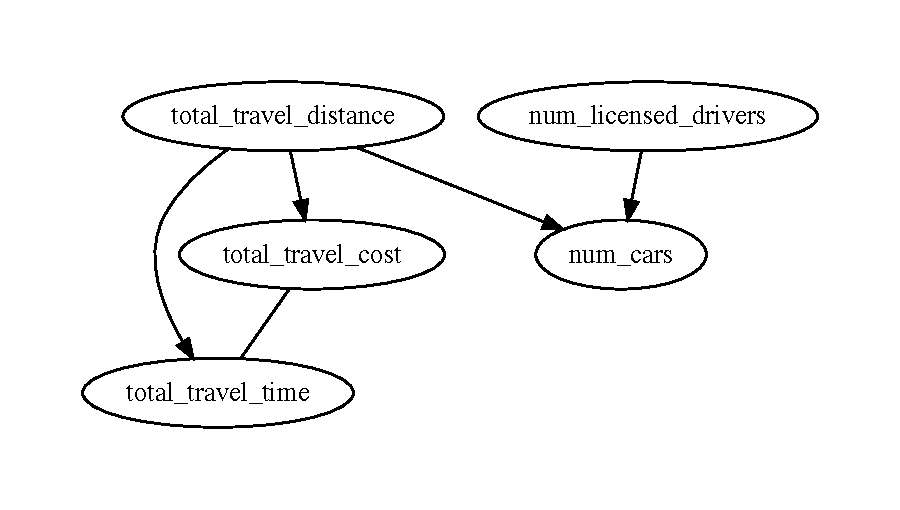
\includegraphics[width=0.5\textwidth]{discovery-example-graph}
   \caption{Result of using the PC algorithm on variables in the drive-alone utility}
   \label{fig:discovery-example-graph}
\end{figure}

Figure \ref{fig:discovery-example-graph} shows the final result of applying the PC algorithm to the variables in our drive-alone utility function.
Two main differences exist between this graph and the example graph shown in Figure \ref{fig:graph-for-testing}.
First, the number of licensed drivers is not independent of the number of automobiles in the household.
The graph discovered via the PC algorithm depicts the number of automobiles in one's household as a function of two variables: the number of licensed drivers that one has in one's household and how far one has to travel to work or to school.
The second major difference is the presence of an undirected edge between travel time and travel cost.
The discovered graph labels travel time and travel cost as dependent, even after conditioning on travel distance.

As described in Section \ref{sec:testing-demonstration}, independence testing foreshadows (indeed, determines) both of these results.
Marginal independence testing showed us that the number of licensed drivers in a household and the number of automobiles in that household are not independent.
Likewise, conditional independence testing revealed that travel cost is not independent of travel time, conditional on travel distance.
Far from being a surprising congruence, we should expect this alignment: conditional and marginal independence testing results are used to generate the graph returned by the PC algorithm.

Relative to manual independence testing, what do we gain from using causal discovery algorithms?
Critically, we gain at least three benefits from causal discovery algorithms.
First, we gain insight into the dependence structure of our variables.
For instance, we recover that the number of licensed drivers causes the number of automobiles, as opposed to the reverse.
Secondly, we gain a greater sense of uncertainty in our causal graphs.
For instance, we can bootstrap our data and look at the distribution of inferred causal graphs.
Moreover, discovered graphs with undirected edges express uncertainty about what-causes-what.
Disclosing and marginalizing over structural uncertainty of this kind is rare in choice modelling, as far as we know.
Lastly, we gain confidence in our results.
Through automated tests, we ensure our results are not based on untested or implausible causal assumptions.
